\section{Flying Tourist Problem evaluation}
\label{sec:ftp_eval}

To demonstrate and quantify the actual benefits of the proposed system, a series of FTP instances were defined, ranging from just 1 city to visit (which corresponds to a round-tri[), up to a total of 20 cities. For each problem instance, several solutions were obtained using four different approaches:
\begin{itemize}
    \item a \textit{pseudo-random} approach, i.e., a closed tour randomly generated that connects all the ;
    \item a \textit{metric nearest-neighbor} heuristic that promotes the nodes proximity to define the traveling route (this approach closely approximates the strategy usually followed by a human solver);
    \item a \textit{regular nearest-neighbor} heuristic using the flight price as the objective function;
    \item the \textit{proposed ACO and SA} meta-heuristics (where the best of these two results is chosen), considering two different objective functions (minimization of the total cost and of the entropy). 
\end{itemize}  

In this experiment, the number of nodes was varied and multiple requests (more than 5) were made for each set of nodes, averaging their results.
In every case, the trip starts and returns to Lisbon (Portugal) and visits a given set of cities, randomly chosen from the following set: 
Abuja, Atlanta, Barcelona, Beijing, Cairo, Casablanca, Dubai, Dublin, Frankfurt, Hong Kong, Istanbul, 
Johannesburg, Kiev, Los Angeles, Madrid, Miami, Moscow, New-York (JFK), Oslo, San Francisco, Sidney, Singapore. The start date was set to be the same for all requests(\textit{1 November 2018}), which, upon the execution of the tests, was 50 days into the future. The waiting period on each city was set to a random value between 1 and 5 days. 


%________________________________________________________________________________________________
%_____________________________ Quantitative evaluation ____________________________________________
%________________________________________________________________________________________________
\subsection{Quantitative evaluation and improvement}
\label{sec:ftp_quantitative_eval}

\begin{table*}
\definecolor{Gray}{gray}{0.9}
\definecolor{green}{rgb}{0,0.5,0}
\definecolor{red}{rgb}{0.75,0,0}
\setlength\tabcolsep{4pt}
\renewcommand{\arraystretch}{1.25}
\centering
\caption{Comparison of different Flying Tourist Problem solutions obtained with distinct algorithms and optimization criteria, considering the \textit{Metric Nearest Neighbor} approach (shaded gray) as reference.} 
\resizebox{1.0\textwidth}{!}{
  \begin{tabular}{l|l|r@{~}r|r@{~}r|r@{~}r|r@{~}r|r@{~}r|r@{~}r|r@{~}r|}
  \label{tab:utility}
                                     & \multicolumn{1}{r}{\#Nodes} 
                                     & \multicolumn{2}{|c}{1} 
                                     & \multicolumn{2}{|c}{3}    
                                     & \multicolumn{2}{|c}{5}    
                                     & \multicolumn{2}{|c}{7}
                                     & \multicolumn{2}{|c}{10}   
                                     & \multicolumn{2}{|c}{15}
                                     & \multicolumn{2}{|c|}{20}   \\
  \hline  
  \multirow{4}{*}{\begin{sideways}\hspace*{-4ex}\textbf{PRICE}\end{sideways}}     
                    & Random            & 635  & 
                                                & 1455 & {\color{red}(+1.2\%)} 
                                                & 2194 & {\color{red}(+7.0\%)} 
                                                & 3436 & {\color{red}(+26.6\%)} 
                                                & 4791 & {\color{red}(+28.8\%)} 
                                                & 7222 & {\color{red}(+63.5\%)} 
                                                & 9154 & {\color{red}(+68.8\%)} \\
                    & \cellcolor{Gray}Metric Nearest Neighbor   
                                                & \cellcolor{Gray}635  & \cellcolor{Gray}
                                                & \cellcolor{Gray}1438 & \cellcolor{Gray}
                                                & \cellcolor{Gray}2051 & \cellcolor{Gray}
                                                & \cellcolor{Gray}2715 & \cellcolor{Gray}
                                                & \cellcolor{Gray}3721 & \cellcolor{Gray}
                                                & \cellcolor{Gray}4417 & \cellcolor{Gray}
                                                & \cellcolor{Gray}5422 & \cellcolor{Gray} \\
                    & Regular Nearest Neighbor  & 635  & 
                                                & 1438 & 
                                                & 1993 & {\color{green}(-2.8\%)} 
                                                & 2553 & {\color{green}(-6.0\%)}
                                                & 3412 & {\color{green}(-8.3\%)}
                                                & 3911 & {\color{green}(-11.5\%)}
                                                & 4678 & {\color{green}(-13.7\%)} \\
                            & Proposed (Price)   & 635  & 
                                                & 1398 & {\color{green}(-2.8\%)}
                                                & 1727 & {\color{green}(-15.8\%)}
                                                & 1911 & {\color{green}(-29.6\%)}
                                                & 2466 & {\color{green}(-33.7\%)}
                                                & 3051 & {\color{green}(-30.9\%)}
                                                & 3699 & {\color{green}(-31.8\%)} \\
                            & Proposed (Entropy)& 876 & {\color{red}(+38.0\%)} 
                                                & 1761 & {\color{red}(+22.5\%)}
                                                & 2203 & {\color{red}(+7.4\%)}
                                                & 2749 & {\color{red}(+1.3\%)}
                                                & 3687 & {\color{green}(-0.9\%)}
                                                & 4123 & {\color{green}(-6.7\%)}
                                                & 4707 & {\color{green}(-13.2\%)} \\ \hline
  \multirow{4}{*}{\begin{sideways}\hspace*{-4ex}\textbf{DURATION}\end{sideways}} 
                            & Random            & 61   & 
                                                & 125  & {\color{red}(+5.0\%)} 
                                                & 183  & {\color{red}(+3.4\%)} 
                                                & 270  & {\color{red}(+31.7\%)} 
                                                & 369  & {\color{red}(+48.2\%)} 
                                                & 497  & {\color{red}(+63.0\%)} 
                                                & 638  & {\color{red}(+92.7\%)}  \\
                            & \cellcolor{Gray}Metric Nearest Neighbor        
                                                & \cellcolor{Gray}61 & \cellcolor{Gray}
                                                & \cellcolor{Gray}119 & \cellcolor{Gray}
                                                & \cellcolor{Gray}177 & \cellcolor{Gray}
                                                & \cellcolor{Gray}205 & \cellcolor{Gray}
                                                & \cellcolor{Gray}249 & \cellcolor{Gray}
                                                & \cellcolor{Gray}305 & \cellcolor{Gray}
                                                & \cellcolor{Gray}331 & \cellcolor{Gray}  \\
                            & Regular Nearest Neighbor       & 61 & 
                                                & 119 & 
                                                & 181 & {\color{red}(+2.3\%)}
                                                & 212 & {\color{red}(+3.4\%)}
                                                & 257 & {\color{red}(+3.2\%)}
                                                & 323 & {\color{red}(+5.9\%)}
                                                & 358 & {\color{red}(+8.2\%)}  \\
                            & Proposed (Price)   & 61 & 
                                                & 121 & {\color{red}(+1.7\%)}
                                                & 151 & {\color{green}(-14.7\%)}
                                                & 179 & {\color{green}(-12.7\%)}
                                                & 258 & {\color{green}(+3.6\%)}
                                                & 292 & {\color{green}(-4.3\%)}
                                                & 319 & {\color{green}(-3.6\%)}  \\
                            & Proposed (Entropy)& 29 & {\color{green}(-52.5\%)}
                                                & 57 & {\color{green}(-52.1\%)}
                                                & 82 & {\color{green}(-53.7\%)}
                                                & 92 & {\color{green}(-55.1\%)}
                                                & 104 & {\color{green}(-58.2\%)}
                                                & 140 & {\color{green}(-54.1\%)}
                                                & 160 & {\color{green}(-51.7\%)} \\ \hline 
  \end{tabular}
}
\end{table*}

The result of the execution of the described test is summarized in Table~\ref{tab:utility}, where both the total flight cost and duration are presented, as a function of the optimization approaches and the number of nodes. This table also presents the observed improvement, relative to the \textit{metric nearest-neighbor} solution, which is used as reference due to its proximity to the human search approach.

%\begin{table}[]
%\centering
%\caption{Solving the Flying Tourist Problem with different algorithms and optimization criteria.} 
%\resizebox{0.5\textwidth}{!}{
%  \begin{tabular}{l|c|cccccccccc}
%  \label{tab:utility}
%  \hline
%                            & N & 1    & 3    & 5    & 7    & 10   & 15   & 20   \\
%  \hline
%  \multirow{4}{*}{C}     & R         & 838  & 1520 & 2089 & 3571 & 4819 & 7289 & 9188 \\
%                            & NN        & 838  & 1512 & 1993 & 2479 & 3229 & 3808 & 4665 \\
%                            & MC        & 838  & 1458 & 1655 & 1928 & 2468 & 3104 & 3721 \\
%                            & ME        & 1158 & 1828 & 2124 & 2521 & 3212 & 3996 & 4704 \\ \hline
%  \multirow{4}{*}{D} & R         & 82   & 125  & 194  & 268  & 378  & 518  & 666  \\
%                            & NN        & 82   & 118  & 157  & 203  & 256  & 313  & 344  \\
%                            & MC        & 82   & 111  & 157  & 181  & 267  & 260  & 325  \\
%                            & ME        & 37   & 58   & 63   & 90   & 105  & 142  & 163 \\ \hline 
%  \end{tabular}
%}
%\end{table}


%\begin{table}[]
%\centering
%\caption{Relative improvement of different optimization algorithms compared to random solution.} 
%\resizebox{0.5\textwidth}{!}{
%    \begin{tabular}{c|c|ccccccc}
%    \label{tab:improvement}
%    \hline
%                       & num nodes & 1     & 3     & 5     & 7     & 10    & 15    & 20    \\
%    \hline
%    \multirow{3}{*}{C} & NN        & 0,0   & -0,5  & -4,6  & -30,6 & -33,0 & -47,8 & -49,2 \\
%                       & MC        & 0,0   & -4,1  & -20,8 & -46,0 & -48,8 & -57,4 & -59,5 \\
%                       & ME        & 38,2  & 20,3  & 1,7   & -29,4 & -33,3 & -45,2 & -48,8 \\ \hline
%    \multirow{3}{*}{D} & NN        & 0,0   & -5,6  & -19,1 & -24,3 & -32,3 & -39,6 & -48,3 \\
%                       & MC        & 0,0   & -11,2 & -19,1 & -32,5 & -29,4 & -49,8 & -51,2 \\
%                       & ME        & -54,9 & -53,6 & -67,5 & -66,4 & -72,2 & -72,6 & -75,5 \\ \hline 
%    \end{tabular}
%}
%\end{table}

The first insight into these results allows a preliminary evaluation of the utility of the proposed system. It can be seen that, for a small number of nodes (1 and 3), the \textit{metric} and \textit{regular} nearest neighbour present the same results. However, for greater instances (5-20) nodes, the \textit{metric} nearest neighbour starts to present worse results when compared to the \textit{regular} variant. The \textit{regular} variant performs better (reducing the cost between $\approx$ $3\%$ and $13\%$) because it always selects the node with the lowest cost. Despite the positive results presented by the \textit{regular} nearest neighbour approach, the proposed meta-heuristics are still capable of improving them. The metaheuristic approach enables the cost to be reduced by an extra 3\% to 25\%, when compared to the \textit{regular} nearest neighbour, and up to a total of 34\%, when compared to the \textit{metric} one. 

%The first insight into these results allows a preliminary evaluation of the utility of the proposed system. It can be seen that, for a small number of nodes (1 and 3), there is no significant improvement relative to the \textit{metric nearest-neighbor} solution. However, when greater instances (5-20 nodes) are considered, this straightforward approach stops presenting good results, while its regular variant (using the flight prices objective function) and the proposed meta-heuristics greatly improve the total flights cost ($\approx$ 3-34\%). However, despite the good results that were presented by the regular nearest neighbour approach (using the flight prices), the proposed meta-heuristics are still capable of improving them ($\approx$ 3-25\%).    


\subsection{Balancing the total flight price and duration}
\label{sec:ftp_obj_func_eval}

It is possible to execute the proposed metaheuristics with different objective functions, as proposed in subsection \ref{sec:ftp}. In particular, it is possible to introduce both the price and flight duration in the objective function (see equation \ref{eq:obj_entropy}). With this approach, a better balance between price and flight duration is envisaged, by minimizing an \textit{entropic} metric defined as a weighted value, where the price and flight duration contribute with 70\% and 30\%, respectively.

%Another implementation of the proposed metaheuristics was also considered that introduce the flight duration in the objective function. With such an alternative implementation, it was envisaged a better balance between price and flight duration, by minimizing an entropy metric defined as a weighted value where the price and flight duration contribute with 70\% and 30\%, respectively.

As it can be observed in Table~\ref{tab:utility}, such an \textit{entropic} minimization leads to significant improvements in the flight duration, although it introduces some penalization in the flight price for a small number of nodes (1-5). However, as the number of nodes increases, the flight price significantly decreases, but it is always higher than that provided by the former price-only meta-heuristics. This happens because the two objective functions (price and duration) can hardly be simultaneously minimized, and thus, a compromise has to be reached. In this case, compromising means slightly increasing the price, to significantly reduce the duration.

This compromise between flight price and duration is also illustrated in Fig.~\ref{fig:cost_vs_time}, which presents the relative duration improvement as a consequence of the increase in price. This figure shows that, in general, increasing the price by around 20\% leads to a decrease in the flight duration by around 50\%, when compared to the price-only metaheuristic approach.

\begin{figure}
  \centering
  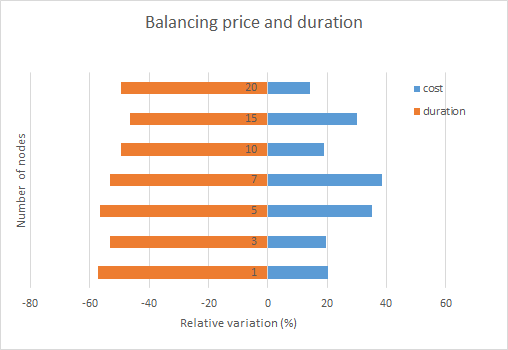
\includegraphics[width=9cm]{./imgs/cost_vs_time.png}
  \caption{Variation of the total flight price and duration when minimizing the entropy objective function.}
  \label{fig:cost_vs_time}  
\end{figure}


\subsection{Impact of the trip start interval}
\label{sec:start_impact}

To evaluate the influence of the trip start interval on the obtained results, the same queries and data sets were used to solve these FTPs using start periods of different lengths.
These results are illustrated in Fig.~\ref{fig:cost_vs_start_period}, where $NN$ refers to the \textit{metric nearest neighbour} heuristic and $M-1$, $M-15$ and $M-31$ represents the proposed meta-heuristic algorithms, with start periods of length 1, 15 and 31 days, respectively. 

The analysis of Fig.~\ref{fig:cost_vs_start_period} shows that increasing the interval of the start date may lead to great improvements, with flight price reductions as high as 15\%, even for medium size instances with up to 20 nodes.  

\begin{figure}[h]
  \centering
  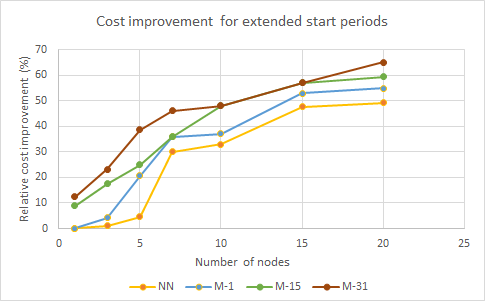
\includegraphics[width=9cm]{./imgs/cost_improvement_startdates.png}
  \caption{Price improvement as a function of the trip start interval.}
  \label{fig:cost_vs_start_period}  
\end{figure}


\subsection{Response time}
\label{sec:response_time}

The response time to a requests depends mostly on two difference procedures: $i$) the data gathering, which is handled by the DMS; and $ii$) the optimization, handled by the OS. This subsection evaluates the response time to a given request, by comparing the relative influence of these two steps. 

As to collect the necessary flight data to a request, it is necessary to communicate with third-party APIs. The module responsible for this is the DMS, which implements a concurrent architecture to make HTTP requests. Figure \ref{fig:dms_factory} illustrates the required time to receive the response to 100 flight queries, using the KIWI flight API. By varying the number of threads, it also shows the speed-up obtained by implementing the concurrent system.

\begin{figure}[h]
  \centering
  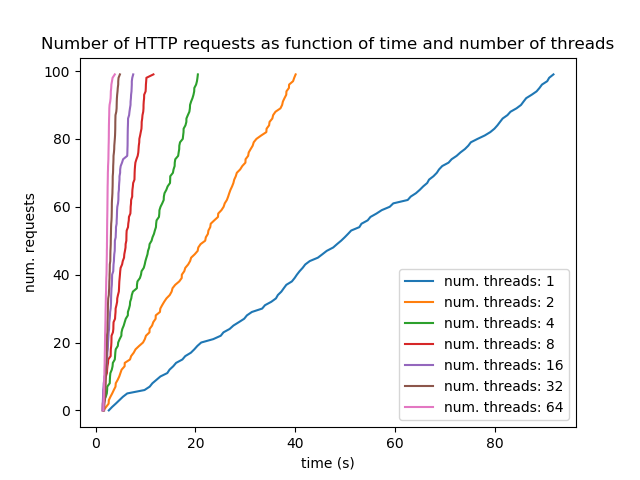
\includegraphics[width=9cm]{./Figures/results/dms_factory.png}
  \caption{Required time to perform 100 HTTP requests to a third-party API, as a function of the number of concurrent requests.}
  \label{fig:dms_factory}  
\end{figure}

Given a serial approach, which corresponds to the case in which there is only one worker thread, the system requires approximately 100 seconds to perform all queries. Thus, the time for the remote API server to respond to one query is, on average, one second. It is possible to increase the number of requests per second, by opting for a concurrent approach. Figure \ref{fig:dms_factory} shows that by performing two concurrent requests, the response time drops to half. As the number of concurrent requests increases, the response time decreases. 

However, this decrease is not always linear. While the first concurrent requests have a very positive effect in the reduction of the response time, this behavior eventually reaches a stagnation point, in which continuing to increase the number of concurrent requests has a negative effect. Thus, it is recommended to be sensible upon defining the number of concurrent requests. Despite this, the proposed DMS allows the collection of 100 requests in less than 5 seconds, which is over 20 times faster than the serial approach.

After collecting the necessary set of flights, the proposed system determines the response to a request by running the appropriate optimization algorithms. Each request is solved using the nearest neighbour heuristic, and the SA and ACO metaheuristics. For each request, it is necessary to run the optimization algorithms for a total of three times, one for each objective function (price, flight duration and entropy). While the nearest neighbour runs until a solution is found, it is possible to define multiple stop criteria for the metaheuristics, as it was referred in section \ref{sec:os_eval}. In this particular evaluation, it was defined that each optimization algorithm may run for a maximum of 1 second, or 10.000 iterations.

As a result, the total time that is necessary to respond to a request, as a function of the number of nodes and length of the start period, is illustrated in figure \ref{fig:response_time}. The analysis of this figure shows that requests with up to 10 nodes are solved in less than 60 seconds. It also shows that the response time increases non-linearly as the number of nodes increases. On the other hand, increasing the length of the start interval has low influence for small instances (up to 10 nodes), but has a significant impact for greater instances.

\begin{figure}
  \centering
  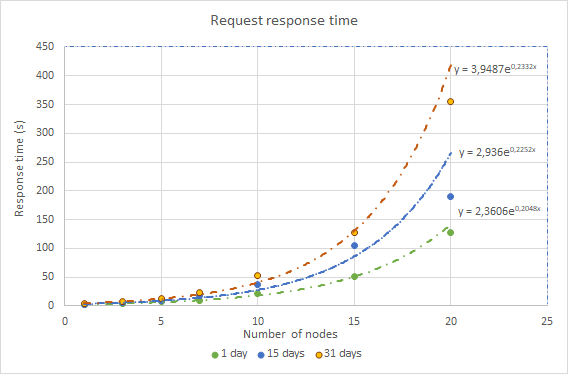
\includegraphics[width=9cm]{./imgs/response_time.png}
  \caption{Total response time to a request, as a function of the number of nodes and length of start period.}
  \label{fig:response_time}  
\end{figure}


% Note that the nearest neighbor and metaheuristics run only after the complete weight matrix is available, which occurs only once the communication with the third-party API is finished. Note also that, after the weight matrix is complete, the nearest neighbor is run first, followed by the metaheuristic for the cost, and finally by the metaheuristic for the entropy. Thus, the completion time of the nearest neighbor, gives a good estimation, or "upper bound", on the time spent communicating with the third-party API, as to obtain the necessary flight data. Figure \ref{fig:kiwi_response_time} presents an accurate illustration of the time spent communicating with the third-party API, as a function of the number of nodes, and the length of the start-period.  



% As to simplify the comprehension of the results presented in table \ref{tab:utility_0}, figure \ref{fig:prices_0} illustrates the improvement of the total flight cost, for the NN and metaheuristic algorithms, relative to the cost of the initial \textit{random} solution. It is worth noting that, for a single node (round flight), the initial random solution, the nearest neighbor, and the metaheuristic, all produce the same result. For 3 nodes, the nearest neighbor does not present relevant improvement, while the metaheuristic already distances itself, presenting around 5\% improvement. For 5 nodes, this difference increases to 20\%, and at 10 nodes it reaches the 50\% mark. Instances with more nodes, 15-20, continue to improve, slowly, up to 60\%.





% We also analyzed the impact of using different objective functions in the optimization process. Instead of optimizing for the total trip cost, the algorithm was set to minimize the entropy, that is, the weighted summation of the flight cost and flight duration. The entropy is set such that the cost weight contributes with 70\%, and the flight duration with the remaining 30\%. After executing the metaheuristic for both objective functions, the total flight cost and duration are compared. The results are illustrated in figure \ref{fig:cost_vs_time}. The inspection of this figure leads to the conclusion that, in general, by increasing the cost by around 20\%, the flight duration decreases to approximately half.


% This series of experiments is completed with the execution of the same problems, this time with a start-period of 31 days. The impact in the solution improvement, relative to the trip cost, can be verified in figure \ref{fig:prices_31}. The analysis of this figure leads to the conclusion that, the selection of an extended start-period, as opposed to a single date, leads to a higher increase in the total savings. For the round flight, the improvement of the metaheuristic is around 10\%. This is because the random and the nearest neighbor solution consider a single start date for the solution construction process. Other small instances, with 3 and 5 nodes, present much higher improvements than those with a single start date, ranging from 20-40\%, as opposed to just 5-20\%. For bigger problem instances, the effect of increasing the start-period is less significant, but it exists, providing an improvement of up to 65\%.





